\section{Secret Sharing}
In this section we look at theory behind secret sharing. Secret sharing is a method for splitting a secret into shares and distributing each shares among a group of participants. None of the participants, on there own, knows any information about the secret from there given share, but by pooling a sufficient number of shares together the secret can be reconstructed. \\

\noindent
The basic model for secret sharing, as described above can be divide into two parts. 

\begin{description}
    \item[Distribution] Where the dealer divided the secret into shares and distributing these shares among a group of participants 
    \item[Reconstruction] Where the secret is reconstructed, given enough participants is pooling there induvidiel shares together. 
\end{description}

\noindent
There are several secret sharing schemes, but we will only be looking at the one used in the electric voting protocol, which is Shamir secret sharing.

\subsection{Shamir Secret Sharing}
The PVSS protocol uses secret sharing as tool to distributes pieces of information. Basically it is about hiding information in a polynomial \begin{math}p\end{math}. For example, a voter chooses a random polynomial of the degree 1, which is a line. The secret is the evaluation of $p$ in \begin{math}0\end{math}. Each server receive a share, the evaluation of  \begin{math}p\end{math} in some other point. Like as server  1 receives  \begin{math}p(1)\end{math}, server 2 receives \begin{math}p(2)\end{math} and etc. To construct the line we need at most two point. One can see that if we don’t have at least 2 points then the line can be constructed in many ways, which is the same as saying we don’t know the evaluation of \begin{math}p(0)\end{math}.\\ \\
In the general case, the polynomial is chosen to be of degree \textit{t}. The scheme requires we need 
 \begin{math}t+1\end{math} points to reconstruct the secret. This means that if we have \textit{t}-servers they would not be able to obtain anything about the secret. 

\subsubsection{Lagrange interpolation}
In secret sharing the secret is reconstructed using Lagrange interpolation. The idea is that we know some evaluations points. With Lagrange interpolation, we have a formula, with which we can reconstruct the polynomial.
The general formula, Lagrange interpolation, looks like:

\begin{defi}[Lagrange polynomial interpolation]
\begin{math}p(x)=\sum\limits_{i \in C} p(i)\lambda_i(x)\end{math}, where $\lambda_i(x)$ is defined by \begin{math} \lambda_i(x)=\prod\limits_{j\in C,j\neq i}  \frac{x-j}{i-j} \end{math}
\end{defi}

\noindent
In secret sharing scheme each server get some shares ("points") and if there are enough servers then the servers can reconstruct the secret by reconstructing the polynomial. By example we will show how the formula works.  We have a polynomial \textit{p}, where we know the evaluation of some points.

\begin{figure}[H]
    \centering
    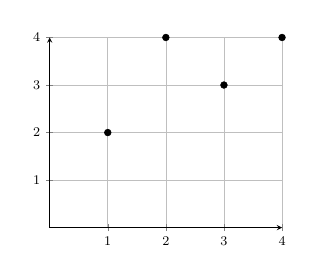
\begin{tikzpicture}[scale=0.6]
    \begin{axis}[
            grid = major,
            xmin=0, xmax=4,
            ymin=0, ymax=4,
            axis lines=center,
            axis on top=true,
            small,
            domain=0:4,
        ]
        \addplot[only marks, color = black, mark = *]
        table[meta=label] {
            x       y       label
            1       2       a
            2       4       a
            3       3       a
            4       4       a
        };
    \end{axis}
    \end{tikzpicture} 
    \caption{polynomial p}
\end{figure}

\noindent
Instead of solving the polynomial, we will start to divide the problem into smaller pieces and solve them one by one. We create a polynomial,\begin{math} \lambda_1, \lambda_2, \lambda_3\end{math} and \begin{math}\lambda_4\end{math}, one for each point from polynomial \textit{p}. These polynomial takes value 1 in one point and 0 in the other points. For example \begin{math} \lambda_1\end{math} takes 1 in 1 and 0 in 2,3 and 4.

\begin{figure}[H]
    \centering
    \captionsetup[subfigure]{labelformat=empty}
    \begin{subfigure}[b]{0.3\textwidth}
        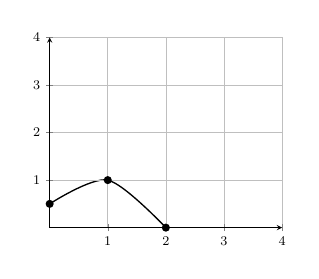
\begin{tikzpicture}[scale=0.6]
        \begin{axis}[
                grid = major,
                xmin=0, xmax=4,
                ymin=0, ymax=4,
                axis lines=center,
                axis on top=true,
                small,
            ]
            \addplot[smooth, thick, color = black, mark = *]
            table[meta=label] {
                x       y       label
                0       0.5     a
                1       1       a
                2       0       a
            };
        \end{axis}
        \end{tikzpicture} 
        \caption{approximately $\lambda_1$}
    \end{subfigure}
    \qquad % <----------------- SPACE BETWEEN PICTURES
    \qquad % <----------------- SPACE BETWEEN PICTURES
    \qquad % <----------------- SPACE BETWEEN PICTURES
    \qquad % <----------------- SPACE BETWEEN PICTURES
    \begin{subfigure}[b]{0.3\textwidth}
        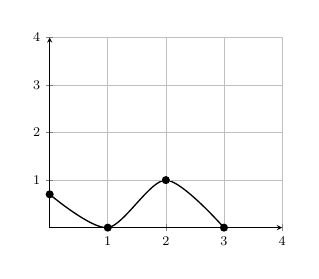
\begin{tikzpicture}[scale=0.6]
        \begin{axis}[
                grid = major,
                xmin=0, xmax=4,
                ymin=0, ymax=4,
                axis lines=center,
                axis on top=true,
                small,
            ]
            \addplot[smooth, thick, color = black, mark = *]
            table[meta=label] {
                x       y       label
                0       0.7     a
                1       0       a
                2       1       a
                3       0       a
            };
        \end{axis}
        \end{tikzpicture} 
        \caption{approximately $\lambda_2$}
    \end{subfigure}
\end{figure}

\noindent
Note that the evaluation in 0 will depend on the secret. For the sake of the drawings it is just an approximately of the point.

\begin{figure}[H]
    \centering
    \captionsetup[subfigure]{labelformat=empty}
    \begin{subfigure}[b]{0.3\textwidth}
        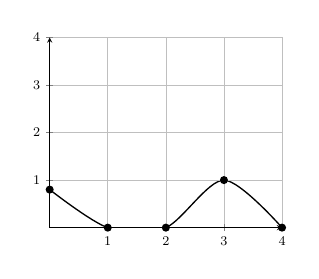
\begin{tikzpicture}[scale=0.6]
        \begin{axis}[
                grid = major,
                xmin=0, xmax=4,
                ymin=0, ymax=4,
                axis lines=center,
                axis on top=true,
                small,
            ]
            \addplot[smooth, thick, color = black, mark = *]
            table[meta=label] {
                x       y       label
                0       0.8     a
                1       0       a
                2       0       a
                3       1       a
                4       0       a
            };
        \end{axis}
        \end{tikzpicture} 
        \caption{approximately $\lambda_3$}
    \end{subfigure}
    \qquad % <----------------- SPACE BETWEEN PICTURES
    \qquad % <----------------- SPACE BETWEEN PICTURES
    \qquad % <----------------- SPACE BETWEEN PICTURES
    \qquad % <----------------- SPACE BETWEEN PICTURES
    \begin{subfigure}[b]{0.3\textwidth}
        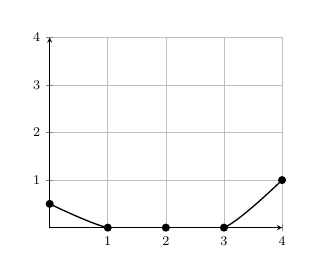
\begin{tikzpicture}[scale=0.6]
        \begin{axis}[
                grid = major,
                xmin=0, xmax=4,
                ymin=0, ymax=4,
                axis lines=center,
                axis on top=true,
                small,
            ]
            \addplot[smooth, thick, color = black, mark = *]
            table[meta=label] {
                x       y       label
                0       0.5     a
                1       0       a
                2       0       a
                3       0       a
                4       1       a
            };           
        \end{axis}
        \end{tikzpicture} 
        \caption{approximately $\lambda_4$}
    \end{subfigure}
\end{figure}

\noindent
To construct the polynomial \begin{math}p\end{math} is to take each polynomials and multiply the corresponding coefficient from \begin{math}p\end{math} and then sum the polynomials together \begin{math}2∙\lambda_1+4∙\lambda_2+3∙\lambda_3+4∙\lambda_4 \end{math}. We started with the \begin{math}\lambda\end{math} polynomial and we ended with four polynomials, which takes value 2,4,3,4 and 0 in the other points. From the sum we see that the value in the first point 2+0+0+0. It is clear this will work in the other points. 

\begin{figure}[H]
    \centering
    \captionsetup[subfigure]{labelformat=empty}
    \begin{subfigure}[b]{0.3\textwidth}
        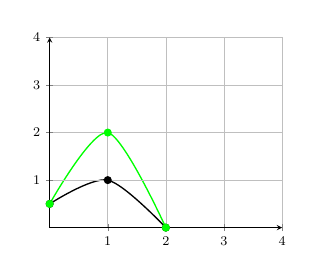
\begin{tikzpicture}[scale=0.6]
        \begin{axis}[
                grid = major,
                xmin=0, xmax=4,
                ymin=0, ymax=4,
                axis lines=center,
                axis on top=true,
                small,
            ]
            \addplot[smooth, thick, color = black, mark = *]
            table[meta=label] {
                x       y       label
                0       0.5     a
                1       1       a
                2       0       a
            };
            \addplot[smooth, thick, color = green, mark = *]
            table[meta=label] {
                x       y       label
                0       0.5     a
                1       2       a
                2       0       a
            };             
        \end{axis}
        \end{tikzpicture} 
        \caption{approximately $\lambda_1$}
    \end{subfigure}
    \qquad % <----------------- SPACE BETWEEN PICTURES
    \qquad % <----------------- SPACE BETWEEN PICTURES
    \qquad % <----------------- SPACE BETWEEN PICTURES
    \qquad % <----------------- SPACE BETWEEN PICTURES
    \begin{subfigure}[b]{0.3\textwidth}
        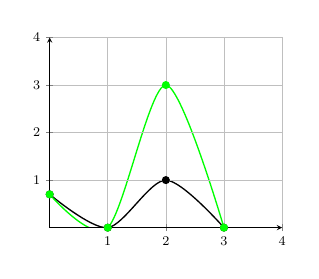
\begin{tikzpicture}[scale=0.6]
        \begin{axis}[
                grid = major,
                xmin=0, xmax=4,
                ymin=0, ymax=4,
                axis lines=center,
                axis on top=true,
                small,
            ]
            \addplot[smooth, thick, color = black, mark = *]
            table[meta=label] {
                x       y       label
                0       0.7     a
                1       0       a
                2       1       a
                3       0       a
            };
            \addplot[smooth, thick, color = green, mark = *]
            table[meta=label] {
                x       y       label
                0       0.7     a
                1       0       a
                2       3       a
                3       0       a
            };             
        \end{axis}
        \end{tikzpicture} 
        \caption{approximately $\lambda_2$}
    \end{subfigure}
\end{figure}

\begin{figure}[H]
    \centering
    \captionsetup[subfigure]{labelformat=empty}
    \begin{subfigure}[b]{0.3\textwidth}
        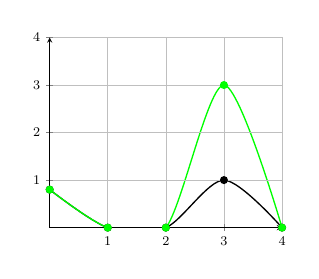
\begin{tikzpicture}[scale=0.6]
        \begin{axis}[
                grid = major,
                xmin=0, xmax=4,
                ymin=0, ymax=4,
                axis lines=center,
                axis on top=true,
                small,
            ]
            \addplot[smooth, thick, color = black, mark = *]
            table[meta=label] {
                x       y       label
                0       0.8     a
                1       0       a
                2       0       a
                3       1       a
                4       0       a
            };
            \addplot[smooth, thick, color = green, mark = *]
            table[meta=label] {
                x       y       label
                0       0.8     a
                1       0       a
                2       0       a
                3       3       a
                4       0       a
            };            
        \end{axis}
        \end{tikzpicture} 
        \caption{approximately $\lambda_3$}
    \end{subfigure}
    \qquad % <----------------- SPACE BETWEEN PICTURES
    \qquad % <----------------- SPACE BETWEEN PICTURES
    \qquad % <----------------- SPACE BETWEEN PICTURES
    \qquad % <----------------- SPACE BETWEEN PICTURES
    \begin{subfigure}[b]{0.3\textwidth}
        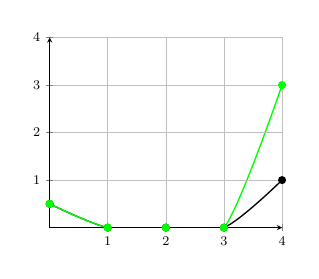
\begin{tikzpicture}[scale=0.6]
        \begin{axis}[
                grid = major,
                xmin=0, xmax=4,
                ymin=0, ymax=4,
                axis lines=center,
                axis on top=true,
                small,
            ]
            \addplot[smooth, thick, color = black, mark = *]
            table[meta=label] {
                x       y       label
                0       0.5     a
                1       0       a
                2       0       a
                3       0       a
                4       1       a
            };
            \addplot[smooth, thick, color = green, mark = *]
            table[meta=label] {
                x       y       label
                0       0.5     a
                1       0       a
                2       0       a
                3       0       a
                4       3       a
            };               
        \end{axis}
        \end{tikzpicture} 
        \caption{approximately $\lambda_4$}
    \end{subfigure}
\end{figure}


\noindent
We will now construct one of the \begin{math}\lambda\end{math}-polynomials by example, by showing it from \begin{math}\lambda_1\end{math} polynomial. 
We have the following points \begin{math}\lambda_1(1)=1, \lambda_1(2)=0, \lambda_1(3)=0 \end{math} and \begin{math} \lambda_1 (4)=0\end{math}. We take the polynomial \begin{math} (x-2)(x-3)(x-4)\end{math}, and we see that if we get correct evaluation in \begin{math}\lambda_1 (2)=0, \lambda_1 (3)=0\end{math} or \begin{math} \lambda_1 (4)=0\end{math}. To get correct evaluation in  \begin{math} \lambda_1 (1)=1\end{math} we divide by \begin{math}-6\end{math} because we see that \begin{math}(1-2)(1-3)(1-4)=-6\end{math} and then we end up with a polynomial \begin{math}\frac{(x-2)(x-3)(x-4)}{(-6)}\end{math} .  The polynomial still satisfies the conditions because when we divide zero with "something" we get zero.  The formula for constructing \begin{math}\lambda_1\end{math} 

\begin{center}
\begin{math} \lambda_1(x)=\prod\limits_{j\in C,j\neq1} \frac{x-j}{1-j} = \frac{x-2}{1-2} \cdot \frac{x-3}{1-3} \cdot \frac{x-4}{1-4}=\frac{(x-2)(x-3)(x-4)}{-6} \end{math}\\
\end{center}

\noindent
\begin{math} \lambda_1\end{math} gives 1 in point 1 and 0 in the other points. What this mean is that in \begin{math} \lambda_1(1)=1\end{math} and all other points  \begin{math}j (2,3,4)\end{math} we have \begin{math} \lambda_1 (j)=0\end{math}. We can construct \begin{math}\lambda_1, \lambda_2, \lambda_3\end{math} and  \begin{math}\lambda_4\end{math} in the same way.

\begin{center}
\begin{math} \lambda_2(x)=\prod\limits_{j\in C,j\neq2} \frac{x-j}{2-j} = \frac{x-1}{2-1} \cdot \frac{x-3}{2-3} \cdot \frac{x-4}{2-4}=\frac{(x-1)(x-3)(x-4)}{-2} \end{math}\\ 

\begin{math} \lambda_3(x)=\prod\limits_{j\in C,j\neq3} \frac{x-j}{3-j} = \frac{x-1}{3-1} \cdot \frac{x-3}{3-2} \cdot \frac{x-4}{3-4}=\frac{(x-1)(x-2)(x-4)}{-2} \end{math}\\ 

\begin{math} \lambda_4(x)=\prod\limits_{j\in C,j\neq4} \frac{x-j}{4-j} = \frac{x-1}{4-1} \cdot \frac{x-3}{4-2} \cdot \frac{x-3}{4-3}=\frac{(x-1)(x-2)(x-3)}{-6} \end{math}\\ 
\end{center}

\noindent
With the knowledge of the evaluation of \begin{math}p(1), p(2), p(3)\end{math} and  \begin{math}p(4)\end{math} we construct the formula for polynomial evaluation in \begin{math}p(0)\end{math}:


\noindent
\begin{infobox}[Applying Lagrange polynomial interpolation for polynomial evaluation in $0$]
We use the formula \begin{math}p(x)=\sum\limits_{i \in C} p(i)\lambda_i(x)\end{math} and we get the evaluation on some polynomial in $0$
\begin{center}
\begin{math}p(0)=p(1)∙\lambda_1+p(2)∙\lambda_2+p(3)∙\lambda_3+p(4)∙\lambda_4=2∙\lambda_1+4∙\lambda_2+3∙\lambda_3+4∙\lambda_4 \end{math}
\end{center}
\label{info:Applying_Lagrange_polynomial_interpolation}
\end{infobox}



\noindent
The idea of constructing the smaller polynomials is that we can reuse them for constructing other polynomials. From the smaller pieces and the evaluation points we can construct the polynomial from Lagrange interpolation. From the secret sharing scheme we know the degree of the polynomial is bounded. Because the voter will share its secret by choosing a random polynomial of the degree at most \textit{t}. That’s a guaranty we have from the scheme. If the degree of $p(x)$ is at most \textit{t} meaning $p(x)\leq t$. Then we need $t+1$ point to reconstruct the $p(x)$. If the degree 1 (line) then we need two points. The parable is where the degree is 2, here we need 3 points to construct
the polynomial.

\begin{figure}[H]
    \centering
    \captionsetup[subfigure]{labelformat=empty}
    \begin{subfigure}[b]{0.3\textwidth}
        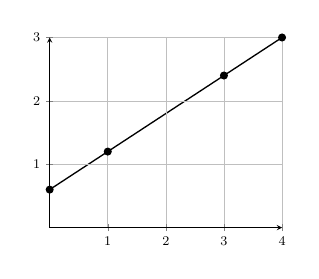
\begin{tikzpicture}[scale=0.6]
        \begin{axis}[
                grid = major,
                xmin=0, xmax=4,
                ymin=0, ymax=3,
                axis lines=center,
                axis on top=true,
                small,
            ]
            \addplot[smooth, thick, color = black, mark = *]
            table[meta=label] {
                x       y       label
                0       0.6     a
                1       1.2     a
                3       2.4     a
                4       3       a
            };
        \end{axis}
        \end{tikzpicture} 
        \caption{polynomial of degree 1}
    \end{subfigure}
    \qquad % <----------------- SPACE BETWEEN PICTURES
    \qquad % <----------------- SPACE BETWEEN PICTURES
    \qquad % <----------------- SPACE BETWEEN PICTURES
    \qquad % <----------------- SPACE BETWEEN PICTURES
    \begin{subfigure}[b]{0.3\textwidth}
        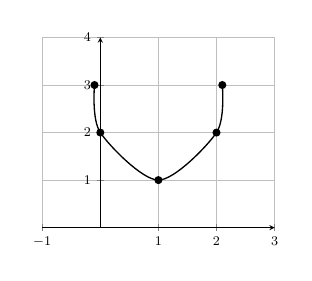
\begin{tikzpicture}[scale=0.6]
        \begin{axis}[
                grid = major,
                xmin=-1, xmax=3,
                ymin=0, ymax=4,
                axis lines=center,
                axis on top=true,
                small,
            ]
            \addplot[smooth, thick, color = black, mark = *]
            table[meta=label] {
                x       y       label
                -0.1    3       a
                0       2       a
                1       1       a
                2       2       a
                2.1     3

            };           
        \end{axis}
        \end{tikzpicture} 
        \caption{polynomial of degree 2}
    \end{subfigure}
\end{figure}


\parahead{In the PVSS protocol} we will use a simplified version of Lagrange interpolation formula. So instead of recovering the polynomium we just recover the evaluation in zero. The following will happen if take the formula \begin{math} \lambda_i(x)=\prod\limits_{j\in C,j\neq i}  \frac{x-j}{i-j} \end{math} and evaluate in zero \begin{math} \lambda_i(0)=\prod\limits_{j\in C,j\neq i}  \frac{0-j}{i-j} = \prod\limits_{j\in C,j\neq i} \frac{j}{j-i} \end{math}. We reduce the formula by evaluating in $0$ and then one can multiply the numerator and denominator by $-1$ and then we get a the above formula.


\noindent
\begin{infobox}[Computing the coefficients for 3 participants]
\begin{math}\lambda_1(0)=\prod\limits_{j\in C,j\neq 1} \frac{2}{2-1}  \cdot  \frac{3}{3-1} =\frac{3}{1} = 3 \end{math}\\
\begin{math}\lambda_2(0)=\prod\limits_{j\in C,j\neq 2} \frac{1}{1-2}  \cdot  \frac{3}{3-2} =\frac{1}{-1} \cdot  \frac{3}{1} =-1 \cdot  3=-3 \end{math}\\
\begin{math}\lambda_3(0)=\prod\limits_{j\in C,j\neq 3} \frac{1}{1-3}  \cdot  \frac{2}{2-3} =\frac{1}{-2} \cdot  \frac{2}{-1} =1 \end{math}\\
\label{info:Computing_the_coefficients}
\end{infobox}

\subsection{Example computation using Shamir Secret Sharing}
We have now explained the basic for secret sharing. This section will show a full concrete computational example on distribution and reconstruction of a secret between 5 participant where we want to tolerate $t=2$ corrupted parties. The computation is computed in $\Z_{11}^*$. The example is that one participant, $p_1$, has a secret, $s=7$ and creates shares to the other participants ($p_2, p_3, p_4, p_5$). Then if $3$ participants combines the shares they will be able to reconstruct the secret. \\

\noindent
First the participant $p_1$ creates a random polynomium, $p(x)$ at degree $t=2$ which is the following polynomium $p(x)=s + a_{1}x+ a_{2}x^2$, where $s=7$ is the secret and $a_{1}=4$ and $a_{2}=1$ is coefficient randomly choosen from $\Z_{11}^*$. The following will show the distribution where $p_1$ create shares to the other parties. In the reconstruction we show how $3$ parties will be able to reconstruct the polynomial and the secret by their shares using Lagrange interpolation.   

\subsubsection{Distribution}
The shares $s_1, s_2, s_3, s_4,s_5$ is computed from $p(x)=7 + 4x+ x^2$ as

\noindent
\begin{alignat*}{4}
s_1&=p(1)&&= 7+4+1 \ &&(mod \ 11) &&=1 \\
s_2&=p(2)&&= 7+8+4 \ &&(mod \ 11) &&=8 \\
s_3&=p(3)&&= 7+12+9 \ &&(mod \ 11) &&=6 \\
s_4&=p(4)&&= 7+16+16 \ &&(mod \ 11) &&=6 \\
s_5&=p(5)&&= 7+20+25 \ &&(mod \ 11) &&=8    
\end{alignat*}


\noindent
Each party now recieve their shares secure. So $p_2= s_2, p_3=s_3, p_4= s_4, p_5= s_5$.

\subsubsection{Reconstruction}
A subset, $3>2$, of participant $p_3, p_4, p_5$ wants to reconstruct the secret by their shares using Lagrange interpolation. First every party computes a polynomial. After that the parties will be able to combine their polynomial and their shares to reconstruct $p(x)$.\\

%------------------------------------------------------------------------------------
\noindent
$p_3$ computes:
%------------------------------------------------------------------------------------


\noindent
\begin{alignat*}{3}
\lambda_3(x)&=\prod\limits_{j\in C,j\neq3} \frac{x-j}{3-j} = \frac{x-4}{3-4} \cdot \frac{x-5}{3-5} =\frac{(x-4)(x-5)}{(3-4)(3-5)}  \\
&= (x^2-9x+20)((3-4)(3-5))^{-1} \ (mod \ 11)
\end{alignat*}

\noindent
The inverse of  $((3-4)(3-5))= 2$ is $6$ since $2 \cdot 6 \ mod \ 11 = 1$. We now have the following polynomial

\noindent
\begin{alignat*}{3}
\lambda_3(x) = (x^2-9x+20)6 \ (mod \ 11) &= (x^2 + 2x+9)6 \ &(mod \ 11) \\
&= 6x^2 + 12x + 54 \ &(mod \ 11) \\
&= 6x^2+x+ 10 \ &(mod \ 11) 
\end{alignat*}

\noindent
We verify the following


\noindent
\begin{alignat*}{6}
\lambda_3(3) &=  6 \cdot 3^2+3+ 10  \ &&(mod \ 11) &&= 67 \ &&(mod \ 11) &&= 1 \\
\lambda_3(4) &=  6 \cdot 4^2+4+ 10  \ &&(mod \ 11) &&= 110 \ &&(mod \ 11) &&= 0 \\
\lambda_3(5) &=  6 \cdot 5^2+5+ 10  \ &&(mod \ 11) &&= 165 \ &&(mod \ 11) &&= 0
\end{alignat*}

%------------------------------------------------------------------------------------
\noindent
$p_4$ computes:
%------------------------------------------------------------------------------------

\noindent
\begin{alignat*}{3}
 \lambda_4(x)&=\prod\limits_{j\in C,j\neq4} \frac{x-j}{4-j} = \frac{x-3}{4-3} \cdot \frac{x-5}{4-5} =\frac{(x-3)(x-5)}{(4-3)(4-5)}\\ 
 &= (x^2-8x+15)((4-3)(4-5))^{-1} \ (mod \ 11)
\end{alignat*}



\noindent
The inverse of  $((4-3)(4-5))= -1$ is $10$ since $-1 \cdot 10 \ (mod \ 11) = 1$. We now have the following polynomial


\noindent
\begin{alignat*}{3}
\lambda_4(x) = (x^2-8x+15)10 \ (mod \ 11) &= (x^2 + 3x+4)10 \ &&(mod \ 11) \\
                                          &= 10x^2 + 8x + 7 \ &&(mod \ 11) 
\end{alignat*}

\noindent
We verify the following

\noindent
\begin{alignat*}{3}
\lambda_4(3) &=  10 \cdot 3^2+24+ 7  \ (mod \ 11) &&= 121 \ (mod \ 11) = 0 \\
\lambda_4(4) &=  10 \cdot 4^2+32+ 7  \ (mod \ 11) &&= 199 \ (mod \ 11) = 1 \\
\lambda_4(5) &=  10 \cdot 5^2+40+ 7  \ (mod \ 11) &&= 297 \ (mod \ 11) = 0 \\
\end{alignat*}




%------------------------------------------------------------------------------------
\noindent
$p_5$ computes:
%------------------------------------------------------------------------------------

\noindent
\begin{alignat*}{3}
 \lambda_5(x)&=\prod\limits_{j\in C,j\neq5} \frac{x-j}{5-j} = \frac{x-3}{5-3} \cdot \frac{x-4}{5-4} =\frac{(x-3)(x-4)}{(5-3)(5-4)} \\
&= (x^2-7x+12)((5-3)(5-4))^{-1} \ (mod \ 11)
\end{alignat*}



\noindent
The inverse of  $((5-3)(5-4))= 2$ is $6$ since $2 \cdot 6 \ mod \ 11 = 1$. We now have the following polynomial

\noindent
\begin{alignat*}{3}
\lambda_5(x)= (x^2-7x+12)6 \ (mod \ 11) &= (x^2 + 4x+1)6 \ &&(mod \ 11) \\
                                        &= 6x^2 + 24x + 6 \ &&(mod \ 11) \\
                                        &= 6x^2 + 2x + 6 \ &&(mod \ 11)
\end{alignat*}

\noindent
We verify the following

\noindent
\begin{alignat*}{6}
\lambda_5(3) &=  6 \cdot 3^2+6+ 6  \ &&(mod \ 11) &&= 66 \ &&(mod \ 11)  &&= 0 \\
\lambda_5(4) &=  6 \cdot 4^2+8+ 6  \ &&(mod \ 11) &&= 110 \ &&(mod \ 11) &&= 0 \\
\lambda_5(5) &=  6 \cdot 5^2+10+6  \ &&(mod \ 11) &&= 166 \ &&(mod \ 11) &&= 1  
\end{alignat*}




\noindent
To construct the polynomial \begin{math}p\end{math} we take each polynomials and multiply by the corresponding shares. More formally we apply \begin{math}p(x)=\sum\limits_{i \in C} p(i)\lambda_i(x)\end{math} to construct the $p(x)$.



\noindent
 \begin{alignat*}{2}
p(x) &= s_3 \lambda_3 (x) + s_4 \lambda_4 (x) + s_5 \lambda_5 (x) &\\
     &= s_3(6x^2+x+ 10) + s_4(10x^2 + 8x + 7)  + s_5(6x^2 + 2x + 6)&\\
     &= (6s_3+10s_4+6s_5)x^2 + (s_3 + 8s_4 + 2s_5)x  + (10s_3 + 7s_4 + 6s_5)&
\end{alignat*} 
   

\noindent
Since the polynomial is of the form $p(x)=s + a_{1}x+ a_{2}x^2$ we have that

\noindent
\begin{alignat*}{2}
s&  = 10s_3 + 7s_4 + 6s_5 \ &&(mod \ 11)  \\
a_1&= s_3 + 8s_4 + 2s_5\ &&(mod \ 11) \\
a_2&= 6s_3+10s_4+6s_5\ &&(mod \ 11) 
\end{alignat*} 

\noindent
We can now replace the variables with shares $s_3=6, s_4=6, s_5=8$

\noindent
\begin{alignat*}{6}
s&  = 10 \cdot 6 + 7 \cdot 6 + 6 \cdot 8 \ &&(mod \ 11)  &&= 150  \ &&(mod \ 11) &&= 7\\
a_1&= 6 + 8 \cdot 6 + 2 \cdot 8 \ &&(mod \ 11) &&= 70  \ &&(mod \ 11) &&= 4\\
a_2&= 6 \cdot 6 +10 \cdot 6+ 6 \cdot 8 \ &&(mod \ 11) &&= 144  \ &&(mod \ 11) &&= 1
\end{alignat*}

\noindent
The reconstruction gives us the final polynomial $p(x)=7 + 4x+ x^2$ and thereby the secret value $7$.


\subsection{Verifiable Secret Sharing (VSS)}
Where the basic model of secret sharing assumes that every participants involved is honest, the VSS requires its participants to prove so. The objective of the VSS is to resisted malicious participants which are defined as \cite{Schoenmakers1999}

\begin{itemize}
    \item Dealer is sending incorrect shares to some or all participants in the distribution phase
    \item Participants is submitting incorrect shares during the reconstruction phase
\end{itemize}

\noindent 
By requiring proof of correctness of the shares, from the participants, in the distribution and the reconstruction phase, the VSS model solves the problem of malicious participants. These proofs is constructed in such a way that only the participants is able to construct and verify the proofs. Where it is a logical requirement that only the participants is able to construct the proofs, it is a different story with the verification. In fact in most case it would be ideal if anybody could validate the proofs. 


\subsection{Public Verifiable Secret Sharing (PVSS)}
In a PVSS schemes it is required that, not only the participants but anybody, is able to validate the shares. It is therefore not assumed that there are private channels between the participants. All communication in PVSS schemes  is done over authenticated public channels using public key encryption, which also means that the secret is only computationally hidden. A common structure for the PVSS protocols is as follows.

\begin{description}
    \item[Initialization] Each participants registers itself and must have a public key.  
    
    \item[Distribution] consists of a distribution and a verification phase
    
    \begin{enumerate}
        \item \textit{Distribution of the shares}
        \begin{enumerate}
            \item \textit{Dealer creates shares}
            \item \textit{Dealer publishes encrypted shares}    
            \item \textit{Dealer publishes a $proof_D$}   
        \end{enumerate}
        \item \textit{Verification of the shares} 
        \begin{enumerate}
            \item \textit{Anybody who knows the public key can verifier the shares}
            \item \textit{If the verification on $proof_D$ fails the dealer fails and the protocol is aborted}  
        \end{enumerate}
    \end{enumerate}
    
    
    \item[Reconstruction] consists of a decryption phase and pooling the shares phase    
        
    \begin{enumerate}
        \item \textit{Decryption of the shares}
         \begin{enumerate}
            \item \textit{The participants decrypt their shares}
            \item \textit{The participants publishes a $proof_{p_{i}}$}  
        \end{enumerate}
        \item \textit{Pooling the shares}  
        \begin{enumerate}
            \item \textit{$proof_{p_{i}}$ are used to exclude dishonest participants}
            \item \textit{Reconstruction of the secret by any qualified set of participants}  
        \end{enumerate}
    \end{enumerate}        

\end{description}

%------------------------------------------------------------------------------------
\subsection{Homomorphic Secret Sharing}
%------------------------------------------------------------------------------------
A homomorphism is a transformation from one algebraic structure into another of the same type so that the structure is preserved. Importantly, this means that for every kind of manipulation of the original data, there is a corresponding manipulation of the transformed data.\\

\noindent 
A homomorphic encryption scheme is a crypto system that allows computations to be performed on data without decrypting it. It is an encrypting scheme which allows computations to be carried out on ciphertext, thus generating an encrypted result which, when decrypted, matches the result of operations performed on the plaintext.

\parahead{Homomorphic Secret Sharing} is a type of secret sharing algorithm in which the secret is encrypted via homomorphic encryption. In the PVSS scheme we use this property that one can sum the shares which are equal to the sum of the secrets.

